%%%%%%%%%%%%%%%%%%%%%%%%%%%%%%%%%%%%%%%%%
% Beamer Presentation
% LaTeX Template
% Version 1.0 (10/11/12)
%
% This template has been downloaded from:
% http://www.LaTeXTemplates.com
%
% License:
% CC BY-NC-SA 3.0 (http://creativecommons.org/licenses/by-nc-sa/3.0/)
%
%%%%%%%%%%%%%%%%%%%%%%%%%%%%%%%%%%%%%%%%%

%----------------------------------------------------------------------------------------
%	PACKAGES AND THEMES
\documentclass[aspectratio=169]{beamer}
\usepackage[portuges]{babel}
\usepackage[utf8]{inputenc}
\usepackage[alf]{abntex2cite}	
\usepackage[portuguese, linesnumbered, vlined, titlenumbered, ruled]{algorithm2e}
\usepackage{beamerthemesplit}
\usepackage{multirow}
\usepackage{scalefnt}

\usepackage{tikz}
\usetikzlibrary{matrix,backgrounds,matrix,positioning,arrows}
\usetikzlibrary{patterns,arrows,decorations.pathreplacing}
% The Beamer class comes with a number of default slide themes
% which change the colors and layouts of slides. Below this is a list
% of all the themes, uncomment each in turn to see what they look like.

%\usetheme{default}
%\usetheme{AnnArbor}
%\usetheme{Antibes}
%\usetheme{Bergen}
%\usetheme{Berkeley}
%\usetheme{Berlin}
%\usetheme{Boadilla}
%\usetheme{CambridgeUS}
%\usetheme{Copenhagen}
%\usetheme{Darmstadt}
%\usetheme{Dresden}
%\usetheme{Frankfurt}
%\usetheme{Goettingen}
%\usetheme{Hannover}
%\usetheme{Ilmenau}
%\usetheme{JuanLesPins}
%\usetheme{Luebeck}
\usetheme{Madrid}
%\usetheme{Malmoe}
%\usetheme{Marburg}
%\usetheme{Montpellier}
%\usetheme{PaloAlto}
%\usetheme{Pittsburgh}
%\usetheme{Rochester}
%\usetheme{Singapore}
%\usetheme{Szeged}
%\usetheme{Warsaw}

% As well as themes, the Beamer class has a number of color themes
% for any slide theme. Uncomment each of these in turn to see how it
% changes the colors of your current slide theme.

%\usecolortheme{albatross}
%\usecolortheme{beaver}
%\usecolortheme{beetle}
%\usecolortheme{crane}
\usecolortheme{dolphin}
%\usecolortheme{dove}
%\usecolortheme{fly}
%\usecolortheme{lily}
%\usecolortheme{orchid}
%\usecolortheme{rose}
%\usecolortheme{seagull}
%\usecolortheme{seahorse}
%\usecolortheme{whale}
%\usecolortheme{wolverine}

%\setbeamertemplate{footline} % To remove the footer line in all slides uncomment this line
%\setbeamertemplate{footline}[page number] % To replace the footer line in all slides with a simple slide count uncomment this line

%\setbeamertemplate{navigation symbols}{} % To remove the navigation symbols from the bottom of all slides uncomment this line


\usepackage{graphicx} % Allows including images
\usepackage{booktabs} % Allows the use of \toprule, \midrule and \bottomrule in tables

%----------------------------------------------------------------------------------------
%	TITLE PAGE
%----------------------------------------------------------------------------------------

\title[Algoritmos de Ordenação por Contagem]{Estrutura de Dados}
\subtitle{Algoritmos de Ordenação por Contagem}
\author[Frederico Santos de Oliveira]{prof. Frederico Santos de Oliveira}
\institute[UFMT]{Universidade Federal de Mato Grosso\\ Instituto de Engenharia}
\date{}
\begin{document}

%------------------------------------------------
\begin{frame}
\titlepage % Print the title page as the first slide

\begin{figure}[!h]
  \centering
  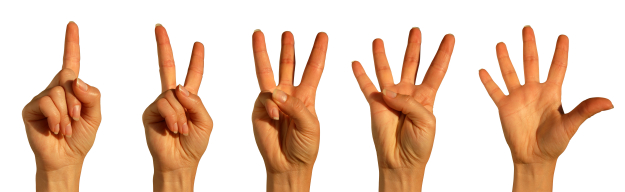
\includegraphics[width=150pt]{imgs/introducao.jpg}
  \label{fig_introducao}
\end{figure}
\end{frame}

%------------------------------------------------

\begin{frame}
\frametitle{Roteiro} % Table of contents slide, comment this block out to remove it
\tableofcontents % Throughout your presentation, if you choose to use \section{} and \subsection{} commands, these will automatically be printed on this slide as an overview of your presentation
\end{frame}

%----------------------------------------------------------------------------------------
%	PRESENTATION SLIDES
%----------------------------------------------------------------------------------------

%------------------------------------------------
\section{Objetivos}

\begin{frame}
\frametitle{Objetivos}

Esta aula tem como objetivos:

\begin{enumerate}
\item Apresentar os métodos de ordenação por contagem:
\begin{itemize}
%  \item Coutingsort
 \item Radixsort
%  \item Bucketsort
 \end{itemize}
\item Exemplificar a execução dos algoritmos.
\end{enumerate}
\end{frame}

%------------------------------------------------

\section{Referências bibliográficas}
  \frame{\frametitle{Referências bibliográficas}
    \bibliographystyle{abntex2-alf}
    \bibliography{referencias}
  }

%------------------------------------------------
\section{Countingsort} % Sections can be created in order to organize your presentation into discrete blocks, all sections and subsections are automatically printed in the table of contents as an overview of the talk
%------------------------------------------------

\begin{frame}
\frametitle{Introdução}
\begin{itemize}
\item Até agora vimos métodos de ordenação que comparam chaves.
\begin{itemize}
\item Esta é uma abordagem genérica que funciona para qualquer tipo de chaves.
\end{itemize}
\item Uma abordagem alternativa para ordenação é processar as chaves por partes.
\begin{itemize}
\item Por exemplo, começamos pelas primeiras letras do nome quando procuramos um nome num catálogo.
\item Não precisamos comprar chaves.
\end{itemize}
\end{itemize}
\end{frame}

\begin{frame}{Algoritmo}{Ideia Geral}
\begin{itemize}
\item Quebrar uma chave em vários pedaços
\begin{itemize}
\item Dígitos de um número em uma dada base (radix)
\item 312 tem os dígitos 3, 1 e 2 na base 10
\item 312 tem os dígitos 100111000 na base 2
\item ``exemplo'' tem 6 caracteres (base 256)
\end{itemize}
\item Ordenar de acordo com o primeiro pedaço
\begin{itemize}
\item Números cujo dígito mais à esquerda começa com 0 vêm antes de números cujo dígito mais à esquerda é 1
\end{itemize}
\item Podemos ordenar repetindo esse processo para todos os pedaços
\end{itemize}
\end{frame}

\section{Exemplo}

\begin{frame}{Algoritmo}{Ordenando um dígito}
\begin{itemize}
\item Para isso iremos contar quantos elementos existem de cada valor
\end{itemize}
\begin{figure}[!h]
  \centering
  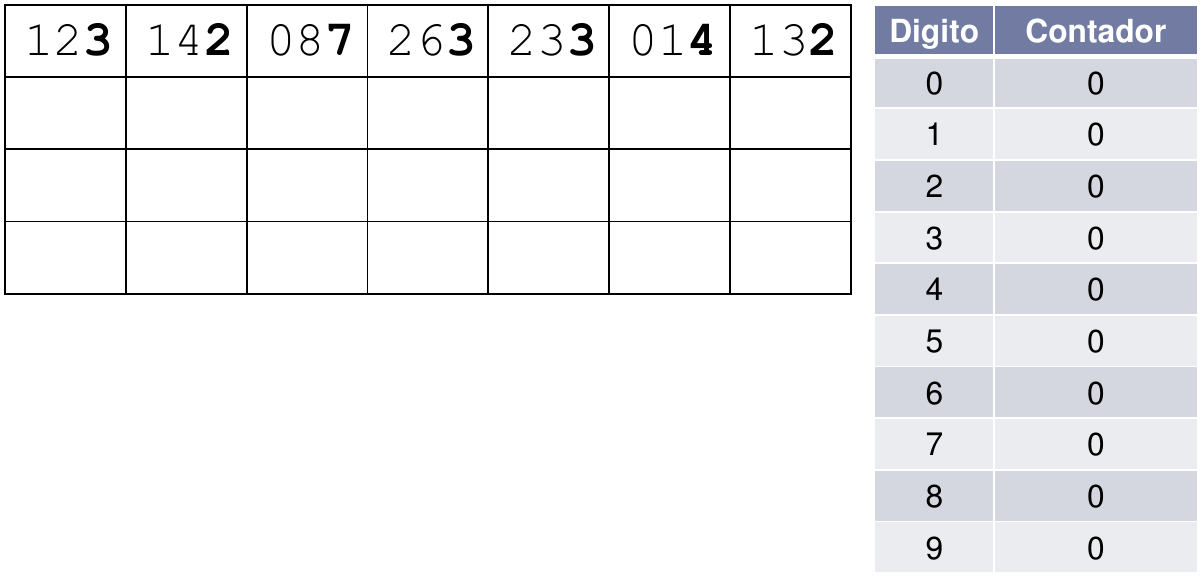
\includegraphics[width=300pt]{imgs/radix1.png}
  \label{radix1}
\end{figure}
\end{frame}

\begin{frame}{Algoritmo}{Ordenando um dígito}
\begin{itemize}
\item Para isso iremos contar quantos elementos existem de cada valor.
\end{itemize}
\begin{figure}[!h]
  \centering
  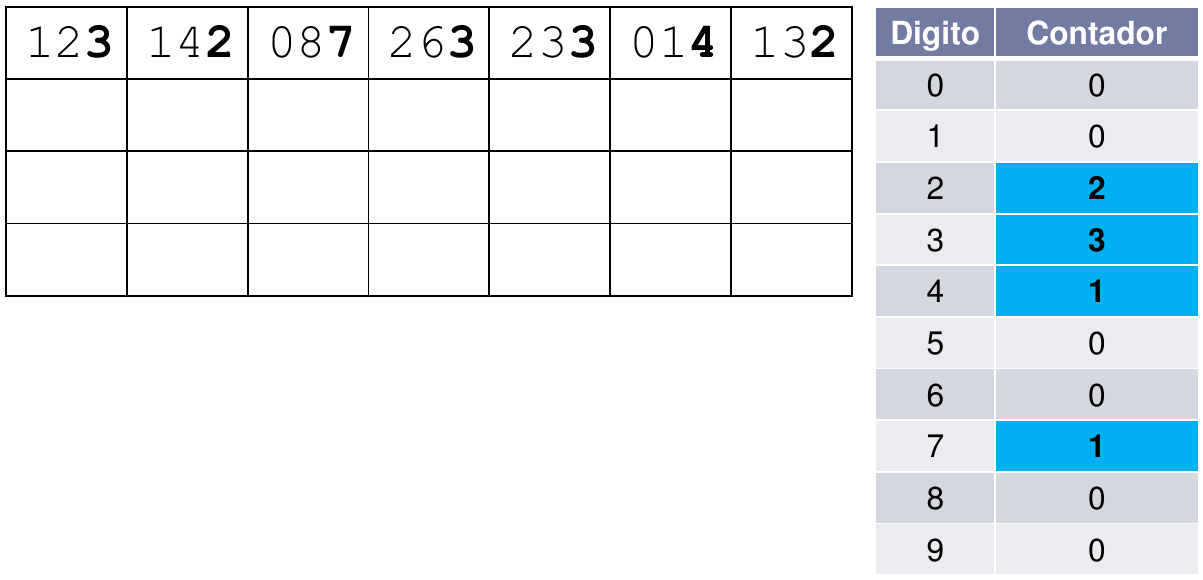
\includegraphics[width=300pt]{imgs/radix2.png}
  \label{radix2}
\end{figure}
\end{frame}

\begin{frame}{Algoritmo}{Ordenando um dígito}
\begin{itemize}
\item  Depois calcular a posição deles no vetor ordenado.
\end{itemize}
\begin{figure}[!h]
  \centering
  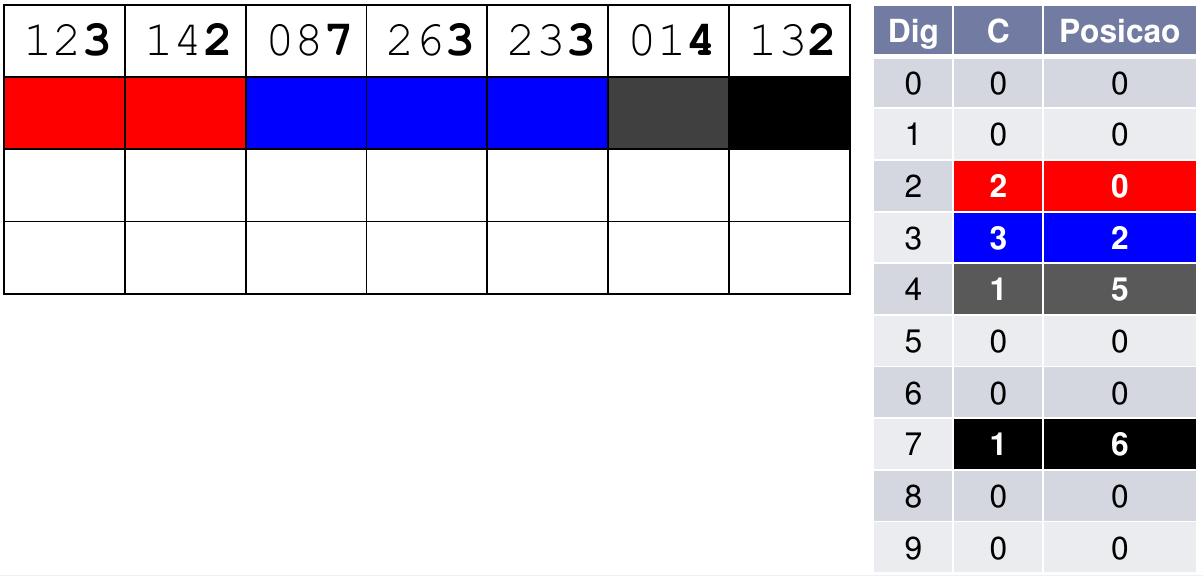
\includegraphics[width=300pt]{imgs/radix3.png}
  \label{radix3}
\end{figure}
\end{frame}

\begin{frame}{Algoritmo}{Ordenando um dígito}
\begin{itemize}
\item E finalmente colocar os elementos em suas posições.
\end{itemize}
\begin{figure}[!h]
  \centering
  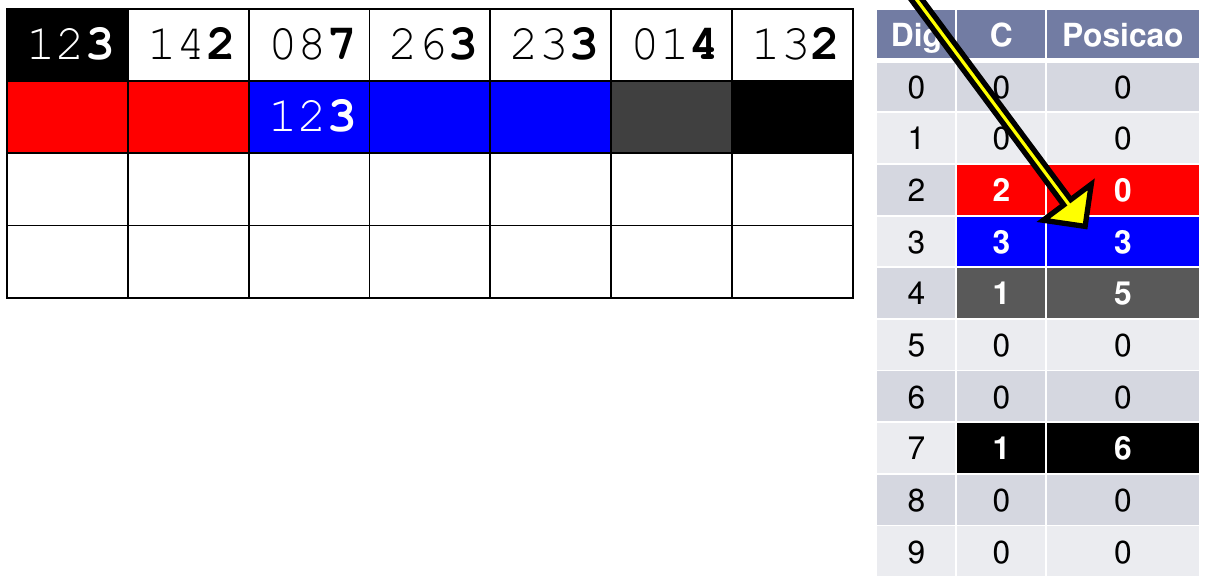
\includegraphics[width=300pt]{imgs/radix4.png}
  \label{radix4}
\end{figure}
\end{frame}

\begin{frame}{Algoritmo}{Ordenando um dígito}
\begin{itemize}
\item Para isso iremos contar quantos elementos existem de cada valor.
\end{itemize}
\begin{figure}[!h]
  \centering
  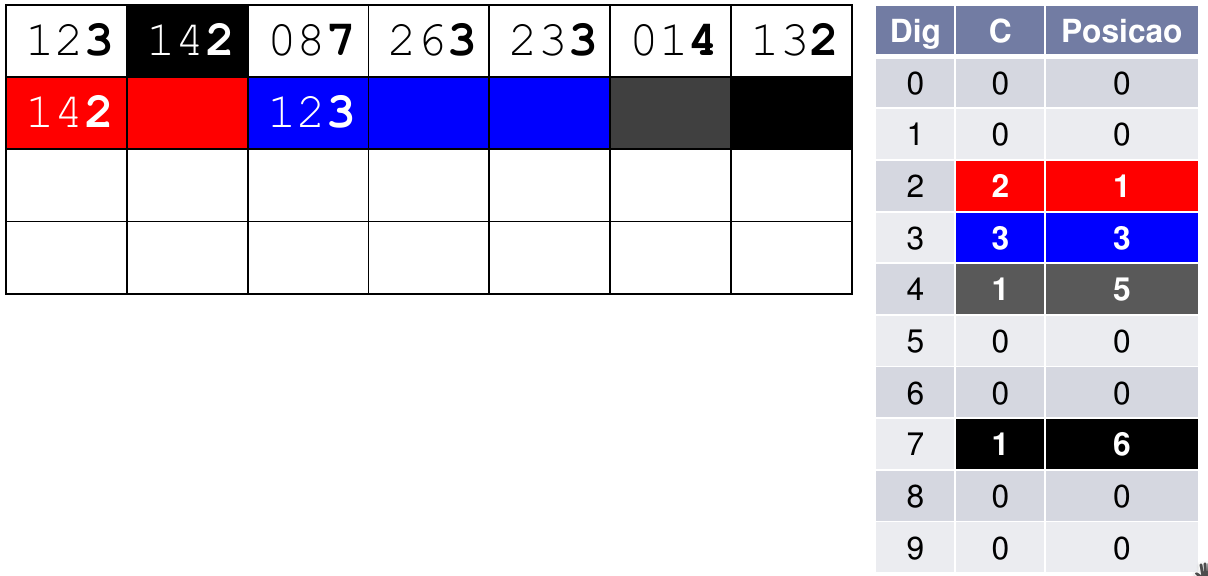
\includegraphics[width=300pt]{imgs/radix5.png}
  \label{radix5}
\end{figure}
\end{frame}


\begin{frame}{Algoritmo}{Ordenando um dígito}
\begin{itemize}
\item Para isso iremos contar quantos elementos existem de cada valor.
\end{itemize}
\begin{figure}[!h]
  \centering
  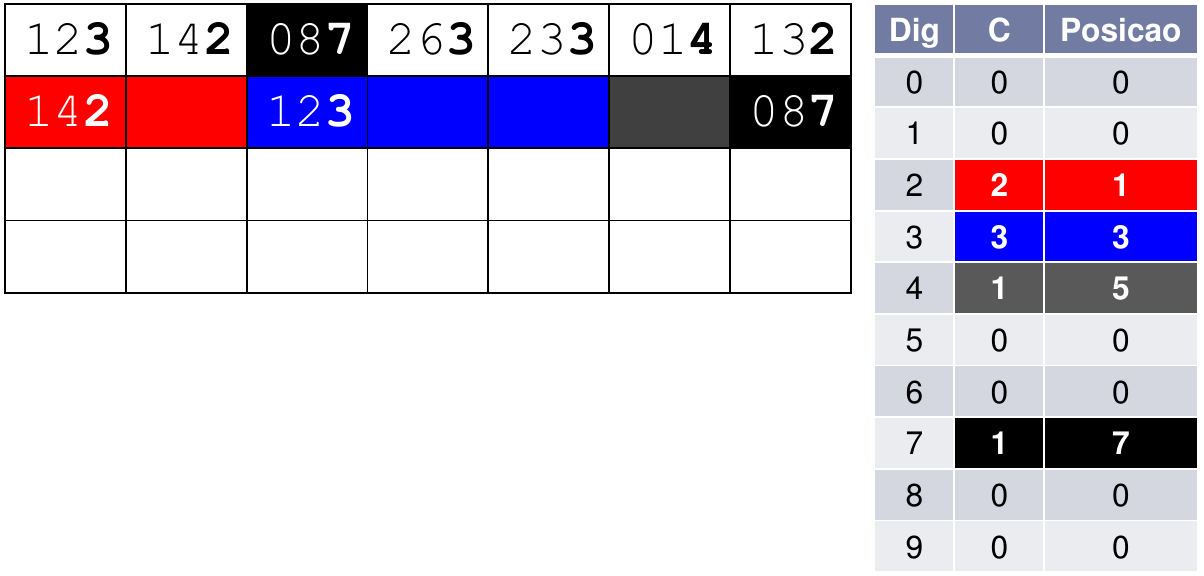
\includegraphics[width=300pt]{imgs/radix6.png}
  \label{radix6}
\end{figure}
\end{frame}


\begin{frame}{Algoritmo}{Ordenando um dígito}
\begin{itemize}
\item Para isso iremos contar quantos elementos existem de cada valor.
\end{itemize}
\begin{figure}[!h]
  \centering
  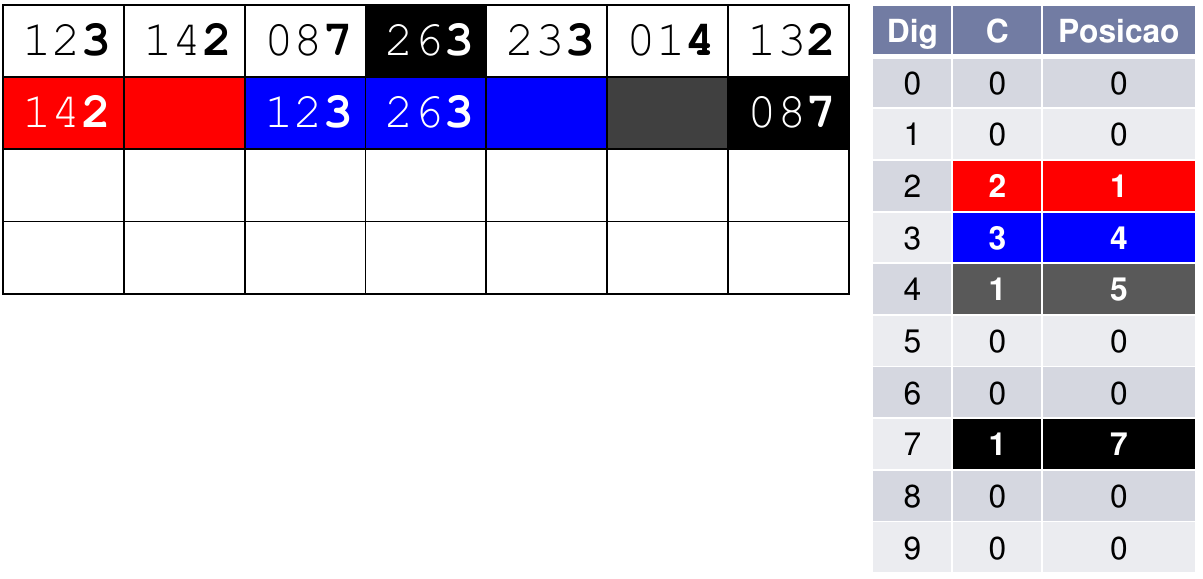
\includegraphics[width=300pt]{imgs/radix7.png}
  \label{radix7}
\end{figure}
\end{frame}


\begin{frame}{Algoritmo}{Ordenando um dígito}
\begin{itemize}
\item Para isso iremos contar quantos elementos existem de cada valor.
\end{itemize}
\begin{figure}[!h]
  \centering
  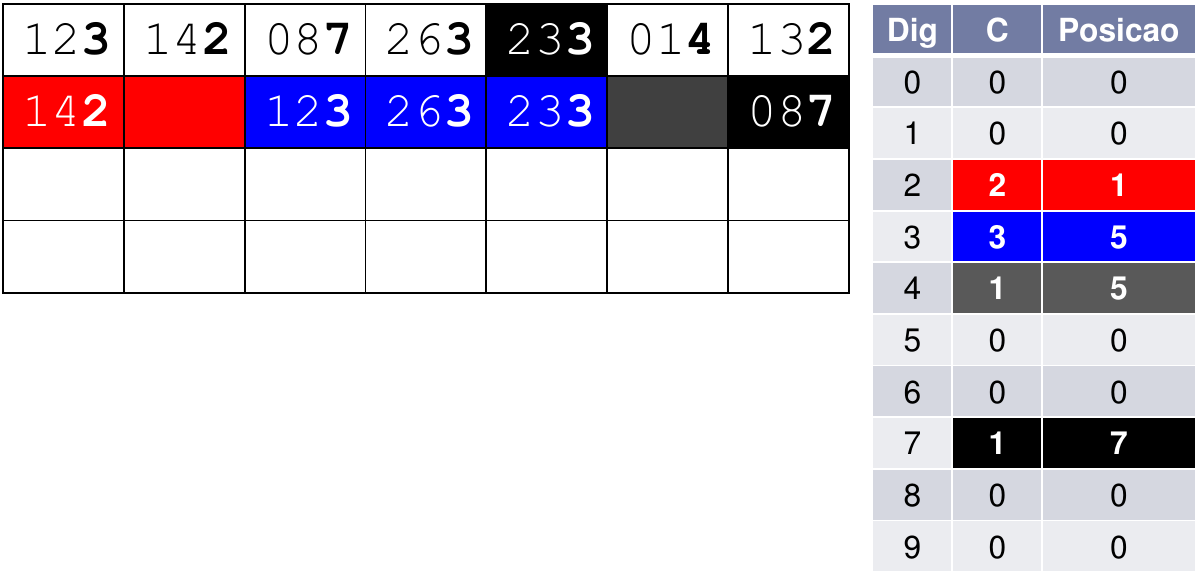
\includegraphics[width=300pt]{imgs/radix8.png}
  \label{radix8}
\end{figure}
\end{frame}


\begin{frame}{Algoritmo}{Ordenando um dígito}
\begin{itemize}
\item Para isso iremos contar quantos elementos existem de cada valor.
\end{itemize}
\begin{figure}[!h]
  \centering
  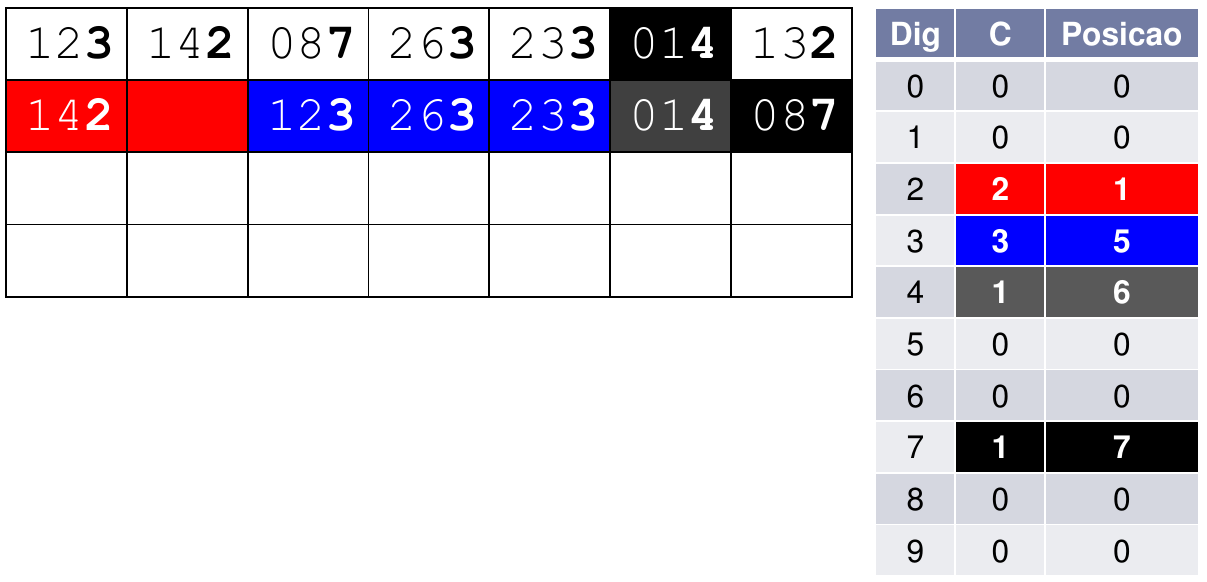
\includegraphics[width=300pt]{imgs/radix9.png}
  \label{radix9}
\end{figure}
\end{frame}


\begin{frame}{Algoritmo}{Ordenando um dígito}
\begin{itemize}
\item Para isso iremos contar quantos elementos existem de cada valor.
\end{itemize}
\begin{figure}[!h]
  \centering
  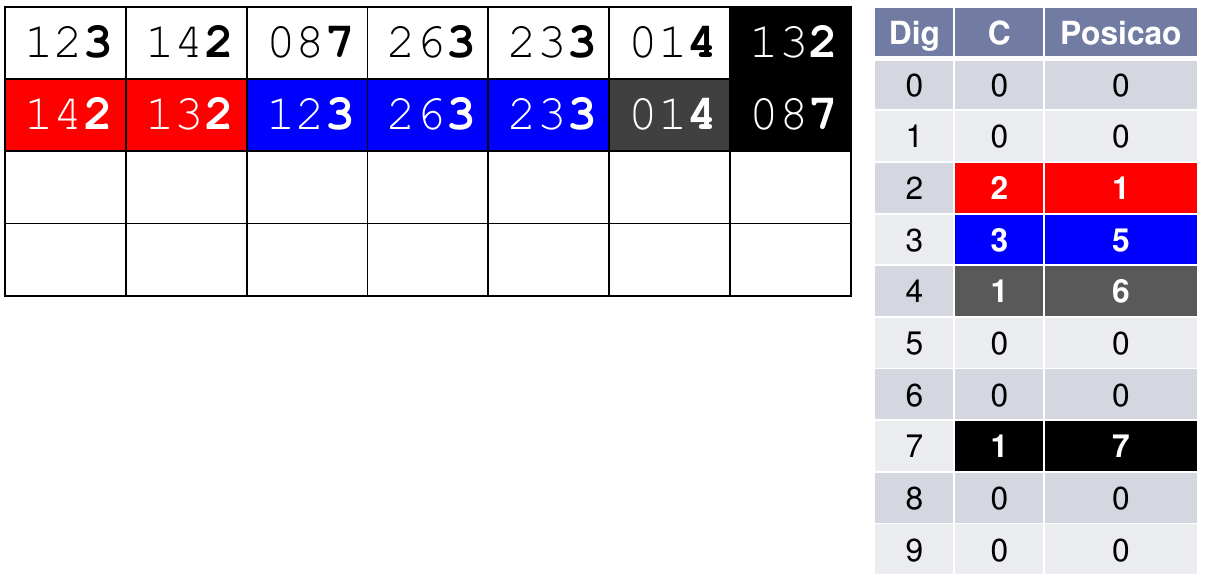
\includegraphics[width=300pt]{imgs/radix10.png}
  \label{radix10}
\end{figure}
\end{frame}


\begin{frame}{Algoritmo}{Ordenando um dígito}
\begin{itemize}
\item Repetimos o mesmo processo para o próximo dígito.
\begin{itemize}
\item Funciona por que o método do contador que usamos anteriormente é estável!
\end{itemize}
\end{itemize}
\begin{figure}[!h]
  \centering
  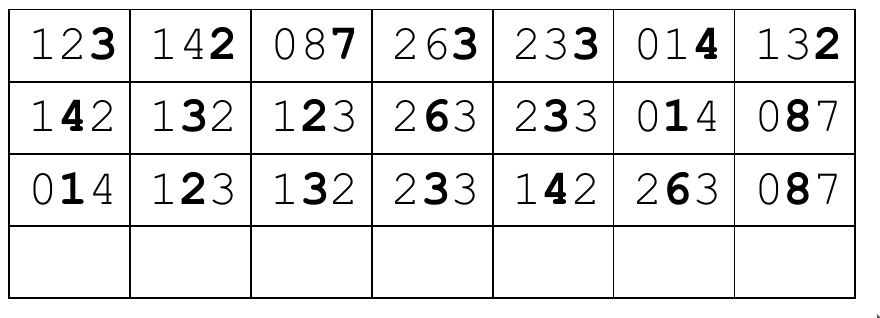
\includegraphics[width=300pt]{imgs/radix11.png}
  \label{radix11}
\end{figure}
\end{frame}

\begin{frame}{Algoritmo}{Ordenando um dígito}
\begin{itemize}
\item Repetimos o mesmo processo para o próximo dígito.
\begin{itemize}
\item Funciona por que o método do contador que usamos anteriormente é estável!
\end{itemize}
\end{itemize}
\begin{figure}[!h]
  \centering
  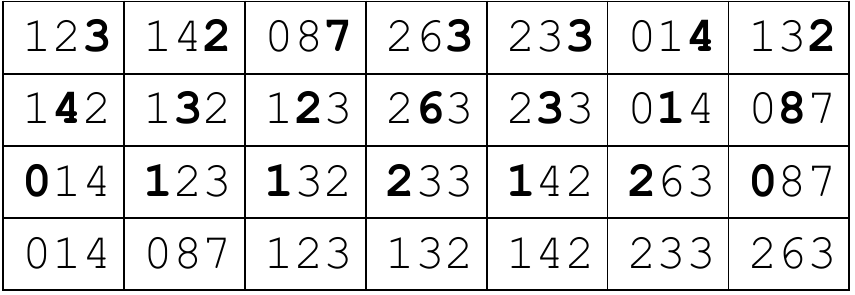
\includegraphics[width=300pt]{imgs/radix12.png}
  \label{radix12}
\end{figure}
\end{frame}

\begin{frame}{Radixsort}{Pseudo-código}
\scalebox{0.8}{
\begin{algorithm}[H]
\caption{Radixsort} 
\label{Radixsort}
\Entrada{Vetor $V[0..n]$, tamanho do vetor $n$, quantidade de dígidos $d$}
\Saida{Vetor $V$ ordenado}
\Inicio{
  \CommentSty{// Cada elemento do vetor possui $d$ dígitos. }\\
  \Para {($i \leftarrow 1$ até $d$)} {
      Ordene $V[0..n]$ pelo dígito $i$ usando um método de ordenação estável (por exexmplo Countingsort) \\
  }

}
\end{algorithm}
}
\end{frame}

\begin{frame}
\frametitle{Conclusão}
\begin{itemize}
\item Vantagens
\begin{itemize}
 \item Não realiza comparações; 
 \item É um algoritmo de ordenação estável;
 \item Se o número de dígitos for pequeno, tem custo computacional $O(n)$.
\end{itemize}
\item Desvantagens
\begin{itemize}
\item Nem sempre é fácil otimizar a inspeção dos dígitos.
\begin{itemize}
\item Depende do hardware.
\end{itemize}
\item Seu uso só é viável se o número de dígitos for pequeno.
\begin{itemize}
\item Em geral o número de dígitos tem crescimento $O(lgn)$.
\end{itemize}
\end{itemize}
\end{itemize}
\end{frame}


%------------------------------------------------

\begin{frame}
\Huge{\centerline{Dúvidas}}

\begin{figure}[!h]
  \centering
  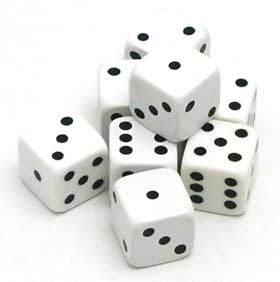
\includegraphics[width=100pt]{imgs/dados.jpg}
  \label{fig_fim}
\end{figure}
\end{frame}
%----------------------------------------------------------------------------------------
\end{document} 